% Options for packages loaded elsewhere
\PassOptionsToPackage{unicode}{hyperref}
\PassOptionsToPackage{hyphens}{url}
%
\documentclass[
  10pt,
  ignorenonframetext,
]{beamer}
\usepackage{pgfpages}
\setbeamertemplate{caption}[numbered]
\setbeamertemplate{caption label separator}{: }
\setbeamercolor{caption name}{fg=normal text.fg}
\beamertemplatenavigationsymbolsempty
% Prevent slide breaks in the middle of a paragraph
\widowpenalties 1 10000
\raggedbottom

\usepackage{amsmath,amssymb}
\usepackage{iftex}
\ifPDFTeX
  \usepackage[T1]{fontenc}
  \usepackage[utf8]{inputenc}
  \usepackage{textcomp} % provide euro and other symbols
\else % if luatex or xetex
  \usepackage{unicode-math}
  \defaultfontfeatures{Scale=MatchLowercase}
  \defaultfontfeatures[\rmfamily]{Ligatures=TeX,Scale=1}
\fi
\usepackage{lmodern}
\usetheme[]{Boadilla}
\usecolortheme{crane}
\useoutertheme{miniframes}
\ifPDFTeX\else  
    % xetex/luatex font selection
\fi
% Use upquote if available, for straight quotes in verbatim environments
\IfFileExists{upquote.sty}{\usepackage{upquote}}{}
\IfFileExists{microtype.sty}{% use microtype if available
  \usepackage[]{microtype}
  \UseMicrotypeSet[protrusion]{basicmath} % disable protrusion for tt fonts
}{}
\makeatletter
\@ifundefined{KOMAClassName}{% if non-KOMA class
  \IfFileExists{parskip.sty}{%
    \usepackage{parskip}
  }{% else
    \setlength{\parindent}{0pt}
    \setlength{\parskip}{6pt plus 2pt minus 1pt}}
}{% if KOMA class
  \KOMAoptions{parskip=half}}
\makeatother
\usepackage{xcolor}
\newif\ifbibliography
\setlength{\emergencystretch}{3em} % prevent overfull lines
\setcounter{secnumdepth}{-\maxdimen} % remove section numbering

\usepackage{color}
\usepackage{fancyvrb}
\newcommand{\VerbBar}{|}
\newcommand{\VERB}{\Verb[commandchars=\\\{\}]}
\DefineVerbatimEnvironment{Highlighting}{Verbatim}{commandchars=\\\{\}}
% Add ',fontsize=\small' for more characters per line
\usepackage{framed}
\definecolor{shadecolor}{RGB}{241,243,245}
\newenvironment{Shaded}{\begin{snugshade}}{\end{snugshade}}
\newcommand{\AlertTok}[1]{\textcolor[rgb]{0.68,0.00,0.00}{#1}}
\newcommand{\AnnotationTok}[1]{\textcolor[rgb]{0.37,0.37,0.37}{#1}}
\newcommand{\AttributeTok}[1]{\textcolor[rgb]{0.40,0.45,0.13}{#1}}
\newcommand{\BaseNTok}[1]{\textcolor[rgb]{0.68,0.00,0.00}{#1}}
\newcommand{\BuiltInTok}[1]{\textcolor[rgb]{0.00,0.23,0.31}{#1}}
\newcommand{\CharTok}[1]{\textcolor[rgb]{0.13,0.47,0.30}{#1}}
\newcommand{\CommentTok}[1]{\textcolor[rgb]{0.37,0.37,0.37}{#1}}
\newcommand{\CommentVarTok}[1]{\textcolor[rgb]{0.37,0.37,0.37}{\textit{#1}}}
\newcommand{\ConstantTok}[1]{\textcolor[rgb]{0.56,0.35,0.01}{#1}}
\newcommand{\ControlFlowTok}[1]{\textcolor[rgb]{0.00,0.23,0.31}{#1}}
\newcommand{\DataTypeTok}[1]{\textcolor[rgb]{0.68,0.00,0.00}{#1}}
\newcommand{\DecValTok}[1]{\textcolor[rgb]{0.68,0.00,0.00}{#1}}
\newcommand{\DocumentationTok}[1]{\textcolor[rgb]{0.37,0.37,0.37}{\textit{#1}}}
\newcommand{\ErrorTok}[1]{\textcolor[rgb]{0.68,0.00,0.00}{#1}}
\newcommand{\ExtensionTok}[1]{\textcolor[rgb]{0.00,0.23,0.31}{#1}}
\newcommand{\FloatTok}[1]{\textcolor[rgb]{0.68,0.00,0.00}{#1}}
\newcommand{\FunctionTok}[1]{\textcolor[rgb]{0.28,0.35,0.67}{#1}}
\newcommand{\ImportTok}[1]{\textcolor[rgb]{0.00,0.46,0.62}{#1}}
\newcommand{\InformationTok}[1]{\textcolor[rgb]{0.37,0.37,0.37}{#1}}
\newcommand{\KeywordTok}[1]{\textcolor[rgb]{0.00,0.23,0.31}{#1}}
\newcommand{\NormalTok}[1]{\textcolor[rgb]{0.00,0.23,0.31}{#1}}
\newcommand{\OperatorTok}[1]{\textcolor[rgb]{0.37,0.37,0.37}{#1}}
\newcommand{\OtherTok}[1]{\textcolor[rgb]{0.00,0.23,0.31}{#1}}
\newcommand{\PreprocessorTok}[1]{\textcolor[rgb]{0.68,0.00,0.00}{#1}}
\newcommand{\RegionMarkerTok}[1]{\textcolor[rgb]{0.00,0.23,0.31}{#1}}
\newcommand{\SpecialCharTok}[1]{\textcolor[rgb]{0.37,0.37,0.37}{#1}}
\newcommand{\SpecialStringTok}[1]{\textcolor[rgb]{0.13,0.47,0.30}{#1}}
\newcommand{\StringTok}[1]{\textcolor[rgb]{0.13,0.47,0.30}{#1}}
\newcommand{\VariableTok}[1]{\textcolor[rgb]{0.07,0.07,0.07}{#1}}
\newcommand{\VerbatimStringTok}[1]{\textcolor[rgb]{0.13,0.47,0.30}{#1}}
\newcommand{\WarningTok}[1]{\textcolor[rgb]{0.37,0.37,0.37}{\textit{#1}}}

\providecommand{\tightlist}{%
  \setlength{\itemsep}{0pt}\setlength{\parskip}{0pt}}\usepackage{longtable,booktabs,array}
\usepackage{calc} % for calculating minipage widths
\usepackage{caption}
% Make caption package work with longtable
\makeatletter
\def\fnum@table{\tablename~\thetable}
\makeatother
\usepackage{graphicx}
\makeatletter
\def\maxwidth{\ifdim\Gin@nat@width>\linewidth\linewidth\else\Gin@nat@width\fi}
\def\maxheight{\ifdim\Gin@nat@height>\textheight\textheight\else\Gin@nat@height\fi}
\makeatother
% Scale images if necessary, so that they will not overflow the page
% margins by default, and it is still possible to overwrite the defaults
% using explicit options in \includegraphics[width, height, ...]{}
\setkeys{Gin}{width=\maxwidth,height=\maxheight,keepaspectratio}
% Set default figure placement to htbp
\makeatletter
\def\fps@figure{htbp}
\makeatother

\setbeamertemplate{footline}
{
\leavevmode%
\hbox{%
\begin{beamercolorbox}[wd=.30\paperwidth,ht=2.25ex,dp=1ex,center]{author in head/foot}%
\usebeamerfont{author in head/foot}\insertshortauthor%
\end{beamercolorbox}%
\begin{beamercolorbox}[wd=.55\paperwidth,ht=2.25ex,dp=1ex,center]{title in head/foot}%
\usebeamerfont{title in head/foot}\insertshorttitle%
\end{beamercolorbox}%
\begin{beamercolorbox}[wd=.15\paperwidth,ht=2.25ex,dp=1ex,center]{date in head/foot}%
\usebeamerfont{date in head/foot}\insertframenumber{} / \inserttotalframenumber
\end{beamercolorbox}}%
}
\makeatletter
\@ifpackageloaded{caption}{}{\usepackage{caption}}
\AtBeginDocument{%
\ifdefined\contentsname
  \renewcommand*\contentsname{Tabla de contenidos}
\else
  \newcommand\contentsname{Tabla de contenidos}
\fi
\ifdefined\listfigurename
  \renewcommand*\listfigurename{Listado de Figuras}
\else
  \newcommand\listfigurename{Listado de Figuras}
\fi
\ifdefined\listtablename
  \renewcommand*\listtablename{Listado de Tablas}
\else
  \newcommand\listtablename{Listado de Tablas}
\fi
\ifdefined\figurename
  \renewcommand*\figurename{Figura}
\else
  \newcommand\figurename{Figura}
\fi
\ifdefined\tablename
  \renewcommand*\tablename{Tabla}
\else
  \newcommand\tablename{Tabla}
\fi
}
\@ifpackageloaded{float}{}{\usepackage{float}}
\floatstyle{ruled}
\@ifundefined{c@chapter}{\newfloat{codelisting}{h}{lop}}{\newfloat{codelisting}{h}{lop}[chapter]}
\floatname{codelisting}{Listado}
\newcommand*\listoflistings{\listof{codelisting}{Listado de Listados}}
\makeatother
\makeatletter
\makeatother
\makeatletter
\@ifpackageloaded{caption}{}{\usepackage{caption}}
\@ifpackageloaded{subcaption}{}{\usepackage{subcaption}}
\makeatother
\ifLuaTeX
\usepackage[bidi=basic]{babel}
\else
\usepackage[bidi=default]{babel}
\fi
\babelprovide[main,import]{spanish}
% get rid of language-specific shorthands (see #6817):
\let\LanguageShortHands\languageshorthands
\def\languageshorthands#1{}
\ifLuaTeX
  \usepackage{selnolig}  % disable illegal ligatures
\fi
\usepackage{bookmark}

\IfFileExists{xurl.sty}{\usepackage{xurl}}{} % add URL line breaks if available
\urlstyle{same} % disable monospaced font for URLs
\hypersetup{
  pdftitle={Tema 06 - Introducción a Quarto},
  pdfauthor={Pedro Albarrán},
  pdflang={es},
  hidelinks,
  pdfcreator={LaTeX via pandoc}}

\title{Tema 06 - Introducción a Quarto}
\subtitle{Técnicas para `Big Data' en Economía - Curso 2023/24\\
Universidad de Alicante}
\author{Pedro Albarrán}
\date{}
\institute{Dpto. de Fundamentos del Análisis Económico. Universidad de
Alicante}
\titlegraphic{
\includegraphics{figure/by-nc-sa.png}}
\logo{
\includegraphics{figure/by-nc-sa2.png}}

\begin{document}
\frame{\titlepage}

\renewcommand*\contentsname{Contenidos}
\begin{frame}[allowframebreaks]
  \frametitle{Contenidos}
  \tableofcontents[hideallsubsections]
\end{frame}
\begin{frame}{El sistema de publicaciones
\href{https://quarto.org/}{Quarto}}
\phantomsection\label{el-sistema-de-publicaciones-quarto}
\begin{columns}[T]
\begin{column}{0.5\textwidth}
\begin{itemize}
\item
  Orientado al análisis de datos \textbf{reproducible}: combina código,
  resultados y comentarios
\item
  Útil como cuaderno de trabajo del código y para \textbf{comunicar}
  resultados en un documento final para tomar decisiones
\end{itemize}
\end{column}

\begin{column}{0.5\textwidth}
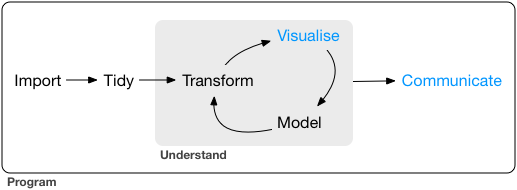
\includegraphics{Tema06_files/mediabag/figure/data-science-communicate.pdf}
\end{column}
\end{columns}

\begin{itemize}
\item
  Instalar Quarto para vuestro sistema operativo desde
  \href{https://quarto.org/docs/get-started/}{aquí}
\item
  La \href{https://quarto.org/docs/guide/}{guía} y
  \href{https://quarto.org/docs/reference/}{referencia} completa de
  Quarto están en su Web
\item
  Un documento de Quarto se renderiza, procesando cada componente
  (código, resultado de ejecutarlo y texto) para producir documentos en
  varios formatos: html, PDF, Word, presentaciones, etc.
\end{itemize}
\end{frame}

\begin{frame}[fragile]{Documentos de Quarto: Crear y Guardar}
\phantomsection\label{documentos-de-quarto-crear-y-guardar}
\begin{itemize}
\item
  Un documento de Quarto se crea a partir de una plantilla en RStudio
  con
  
\includegraphics[width=0.07\textwidth,height=\textheight]{figure/Mas2.jpg}
  o \emph{File \textgreater{} New File \textgreater{} Quarto Document}

  \begin{itemize}
  \tightlist
  \item
    Podemos elegir Título, Autor/a y formato de salida (HTML, por
    defecto)
  \end{itemize}
\end{itemize}

\begin{itemize}
\item
  Se guarda con 
\includegraphics{figure/Guardar.jpg} o con \emph{File
  \textgreater{} Save}, con extensión \texttt{.qmd}
\item
  Se renderiza con
  
\includegraphics[width=0.1\textwidth,height=\textheight]{figure/Render.jpg}
  al formato de salida elegido
\item
  En el botón de engranaje 
\includegraphics{figure/Engranaje.jpg} se
  pueden cambiar algunas opciones

  \begin{itemize}
  \tightlist
  \item
    p.e., dónde se visualiza la salida (en ventana aparte o en RStudio)
  \end{itemize}
\end{itemize}
\end{frame}

\begin{frame}[fragile]{Documentos de Quarto: formato de salida}
\phantomsection\label{documentos-de-quarto-formato-de-salida}
\begin{itemize}
\item
  El renderizado crea un archivo en el mismo directorio donde está el
  archivo de Quarto .qmd
\item
  En el caso de HTML, se crea tanto un archivo con extensión .html como
  un subdirectorio del mismo nombre con componentes necesarios (ej.,
  imágenes, css)

  \begin{itemize}
  \tightlist
  \item
    solo podemos visualizar correctamente el archivo .html en cualquier
    navegador si copiamos a otro lugar tanto el .html como el
    subdirectorio
  \end{itemize}
\item
  Para crear PDFs, se necesita una distribución de
  \href{https://es.wikipedia.org/wiki/LaTeX}{LaTeX}: instala una
  escribiendo en la pestaña de ``Terminal'' (a la derecha de la
  consola):
\end{itemize}

\begin{Shaded}
\begin{Highlighting}[]
\NormalTok{quarto install tool tinytex}
\end{Highlighting}
\end{Shaded}
\end{frame}

\begin{frame}[fragile]{Documentos de Quarto: Texto con Markdown}
\phantomsection\label{documentos-de-quarto-texto-con-markdown}
\begin{itemize}
\item
  Los componentes de texto están escritos en Markdown: un conjunto
  ligero de convenciones para archivos de texto sin formato. Por
  ejemplo,

  \begin{itemize}
  \item
    todo lo escrito entre dos * como \texttt{**Hola**} se renderiza en
    negritas
  \item
    se utiliza \# para indicar encabezados de secciones
  \end{itemize}
\item
  En el menú de ayuda tenemos una descripción completa (\emph{Markdown
  quick reference}) y ``chuletas'' (\emph{Cheatsheets})
\item
  También son útiles
  \href{https://quarto.org/docs/authoring/markdown-basics.html}{la web
  de Quarto} y este \href{https://bookdown.org/yihui/rmarkdown/}{libro
  online}.
\end{itemize}

\begin{itemize}
\tightlist
\item
  RStudio incorpora un \textbf{editor visual} de documentos de Quarto,
  similar a un procesador de texto
\end{itemize}
\end{frame}

\begin{frame}{Editor Visual de Quarto en RStudio}
\phantomsection\label{editor-visual-de-quarto-en-rstudio}
\begin{itemize}
\item
  En documentos .qmd, se puede elegir entre editar la fuente
  (\emph{source}) de Markdown, como texto sencillo, o editar el
  documento de forma Visual en 
\includegraphics{figure/Visual.jpg}
\item
  En el modo visual, en esa misma \textbf{barra de herramientas} se
  tienen accesos a

  \begin{itemize}
  \tightlist
  \item
    formatos de texto (negritas, cursivas, encabezamientos) y listas
  \item
    insertar enlaces, imágenes, notas a pie de página, tablas
  \item
    incluir ecuaciones (en
    \href{https://www.latex4technics.com/}{LaTeX})
  \item
    también insertar directamente código HTML, comentarios, etc.
  \end{itemize}
\item
  Se puede configurar la corrección ortográfica en \emph{Tools
  \textgreater{} Global Options \textgreater{} Spelling}:
  agregar/seleccionar el diccionario de Español
\end{itemize}
\end{frame}

\begin{frame}[fragile]{Formato en la cabecera: el bloque \texttt{YAML}}
\phantomsection\label{formato-en-la-cabecera-el-bloque-yaml}
\begin{itemize}
\tightlist
\item
  Al \textbf{principio del documento}, entre dos líneas con
  \texttt{-\/-\/-}, se pueden especificar varias opciones del documento:
  título, autor, fecha, formato de salida
\end{itemize}

\begin{itemize}
\item
  Los formatos de salida son \texttt{html}, \texttt{pdf}, \texttt{docx}
  (y otros en \emph{Quarto Presentations})
\item
  También se especifican opciones globales del documento, algunas
  \emph{específicas} de cada tipo de salida (ver la referencia para
  \href{https://quarto.org/docs/reference/formats/html.html}{\texttt{html}}
  y otros formatos)

\begin{verbatim}
  ---
  title: "Título"
  author: Autor 
  date: 15-octubre-2023
  format:
    html:
      toc: true              # índice
      number-sections: true  # secciones numeradas
      embed-resources: true  # archivo html autocontenido
      theme: united          # más temas: https://bootswatch.com/3/
  ---
\end{verbatim}
\end{itemize}
\end{frame}

\begin{frame}[fragile]{Fragmentos o celdas de código }
\phantomsection\label{fragmentos-o-celdas-de-cuxf3digo}
\begin{itemize}
\item
  Insertamos código en medio del texto con el icono (visual)
  
\includegraphics{figure/Code.jpg}
\item
  Si pulsamos 
\includegraphics{figure/Code.jpg}, escribimos \texttt{r} y
  luego un código, el documento de salida incluirá el resultado de
  ejecutar el código
\end{itemize}

\pause

\begin{itemize}
\item
  Podemos incluir un fragmento de código (de varias líneas), con
  
\includegraphics{figure/Insert_codechunk.png}, en el desplegable
  
\includegraphics{figure/InsertVisual.png} o
  \texttt{Ctrl\ +\ Alt\ +\ I}
\item
  Se puede personalizar cómo se muestran varios aspectos del código y de
  sus resultados

  \begin{itemize}
  \item
    bien para una celda concreta de código, incluyendo
    \href{https://quarto.org/docs/reference/cells/cells-knitr.html}{opciones
    de celda}
  \item
    o para todo el documento en la cabecera: las opciones de
    \texttt{html} están en la sección de código de
    \href{https://quarto.org/docs/reference/formats/html.html}{su
    referencia} (y similar para otros formatos)
  \end{itemize}
\end{itemize}
\end{frame}

\begin{frame}[fragile]{Opciones para una celda de código}
\phantomsection\label{opciones-para-una-celda-de-cuxf3digo}
\begin{itemize}
\item
  Las opciones se incluyen al principio de una celda precedidas por
  \texttt{\#\textbar{}}
\item
  Se muestra el código en la salida con la opción \texttt{echo:\ true}
  (o no con \texttt{echo:\ false})
\item
  Con la opción \texttt{eval:\ false}, el código se ejecuta: los
  resultados de ejecutarlo están disponibles y pueden mostrarse (o no
  con \texttt{eval:\ false})

  \begin{itemize}
  \tightlist
  \item
    Si un fragmento no se evalua, sus resultados no están para otras
    celdas posteriores (p.e., cargamos datos o una biblioteca para usar
    luego)
  \end{itemize}
\item
  Incluimos los resultados del código con \texttt{output:\ true}
\end{itemize}

\begin{itemize}
\item
  También se pueden mostrar (o no) los mensajes, errores y avisos de
  ejecutar un código con las opciones \texttt{message}, \texttt{error} y
  \texttt{warning}, respectivamente.
\item
  La lista completa de opciones
  \href{http://yihui.name/knitr/options/}{aquí}
\end{itemize}
\end{frame}

\begin{frame}[fragile]{Opciones para una celda de código (cont.)}
\phantomsection\label{opciones-para-una-celda-de-cuxf3digo-cont.}
\begin{itemize}
\item
  \emph{Cómo} mostrar resultado

  \begin{itemize}
  \tightlist
  \item
    \texttt{results:\ hide} (no mostrar)
  \item
    \texttt{results:\ hold} (mostrar todo, no el resultado de cada
    línea)
  \end{itemize}
\item
  \texttt{include:\ false} no incluye ni el código ni su resultado, pero
  se evalúa
\item
  \texttt{label}: etiqueta para identificar la celda
\item
  \texttt{code-fold:\ true} oculta el código pero da opción a mostrarlo
\end{itemize}

\begin{itemize}
\item
  \texttt{fig-cap} y \texttt{tbl-cap} para los títulos
\item
  \emph{Cómo} mostrar los gráficos: \texttt{fig-show}

  \begin{itemize}
  \tightlist
  \item
    las opciones \texttt{hide} y \texttt{hold} son como en
    \texttt{results}
  \item
    \texttt{animate} concatena varios gráficos en una animación
  \end{itemize}
\end{itemize}
\end{frame}

\begin{frame}[fragile]{Opciones para una celda de código (y 3)}
\phantomsection\label{opciones-para-una-celda-de-cuxf3digo-y-3}
\begin{itemize}
\item
  \texttt{fig-width} y \texttt{fig-height}: dimensiones (reales, en
  pulgadas) de una figura
\item
  \texttt{out-width} y \texttt{out-height}: ídem en el documento de
  salida (\% de las reales)
\item
  \texttt{fig-align}: mostrar la figura centrada o alineada a derecha o
  izquierda
\item
  \texttt{layout-ncol}: en cuantas columnas se componen los resultados
\end{itemize}

\begin{Shaded}
\begin{Highlighting}[]
\InformationTok{\textasciigrave{}\textasciigrave{}\textasciigrave{}\{r\}}
\InformationTok{\#| layout{-}ncol: 2}
\InformationTok{\#| fig{-}show: hold}
\InformationTok{ggplot(data = cars) + geom\_histogram(aes(x = speed))  \# en la izquierda}
\InformationTok{ggplot(data = cars) + geom\_histogram(aes(x = dist))   \# en la derecha}
\InformationTok{\textasciigrave{}\textasciigrave{}\textasciigrave{}}
\end{Highlighting}
\end{Shaded}

\begin{figure}

\begin{minipage}{0.50\linewidth}
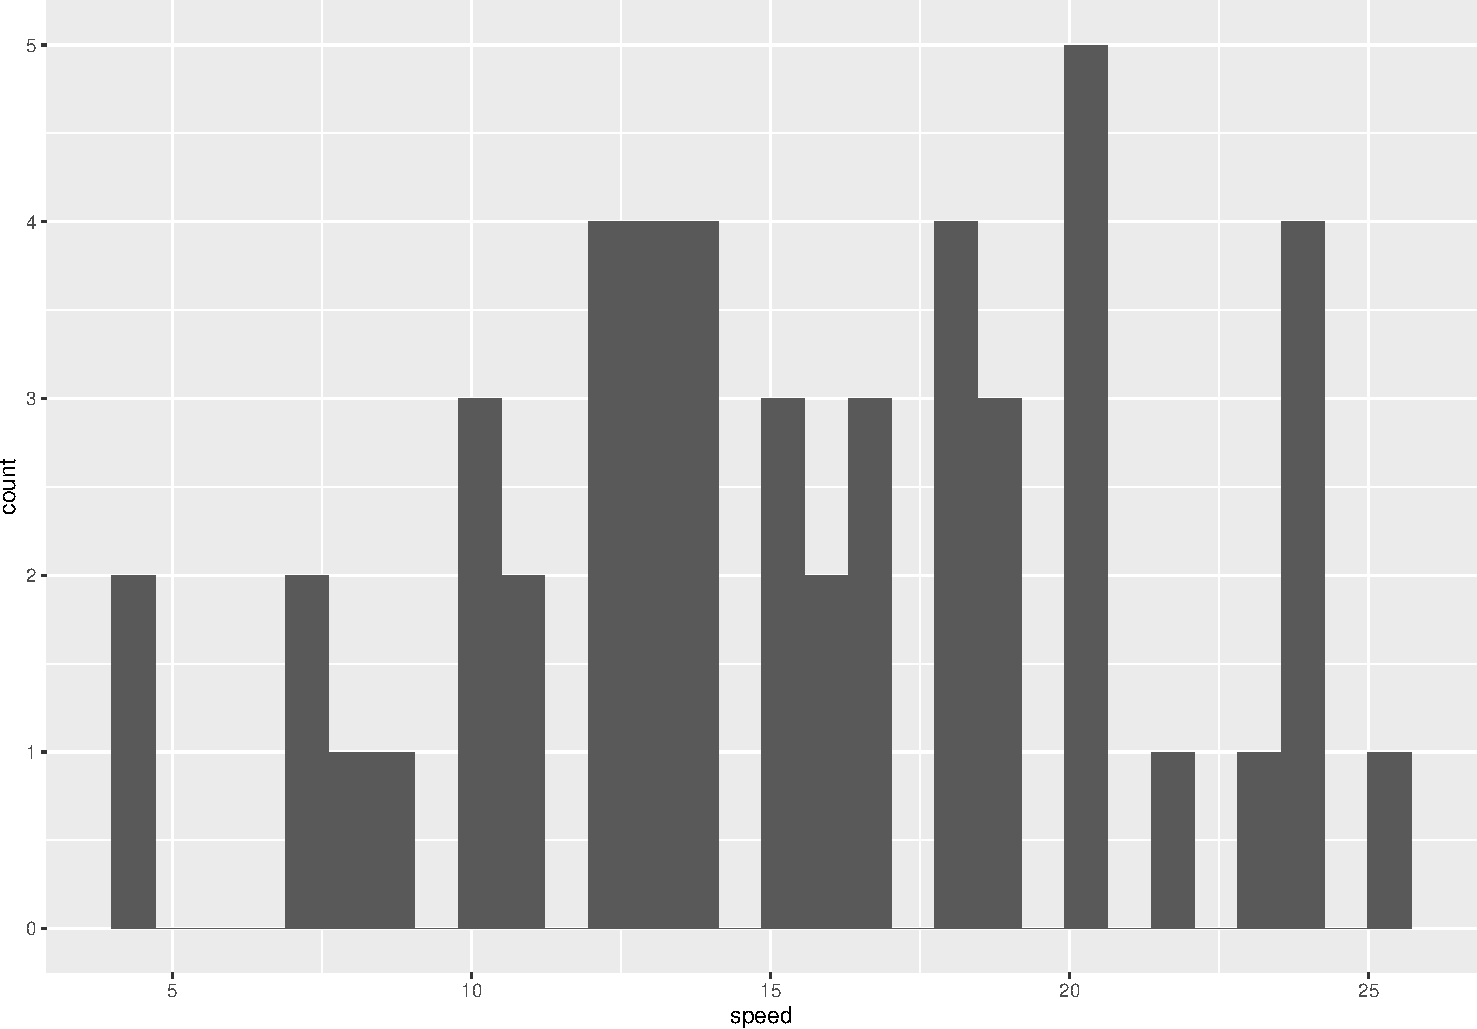
\includegraphics{Tema06_files/figure-beamer/unnamed-chunk-2-1.pdf}\end{minipage}%
%
\begin{minipage}{0.50\linewidth}
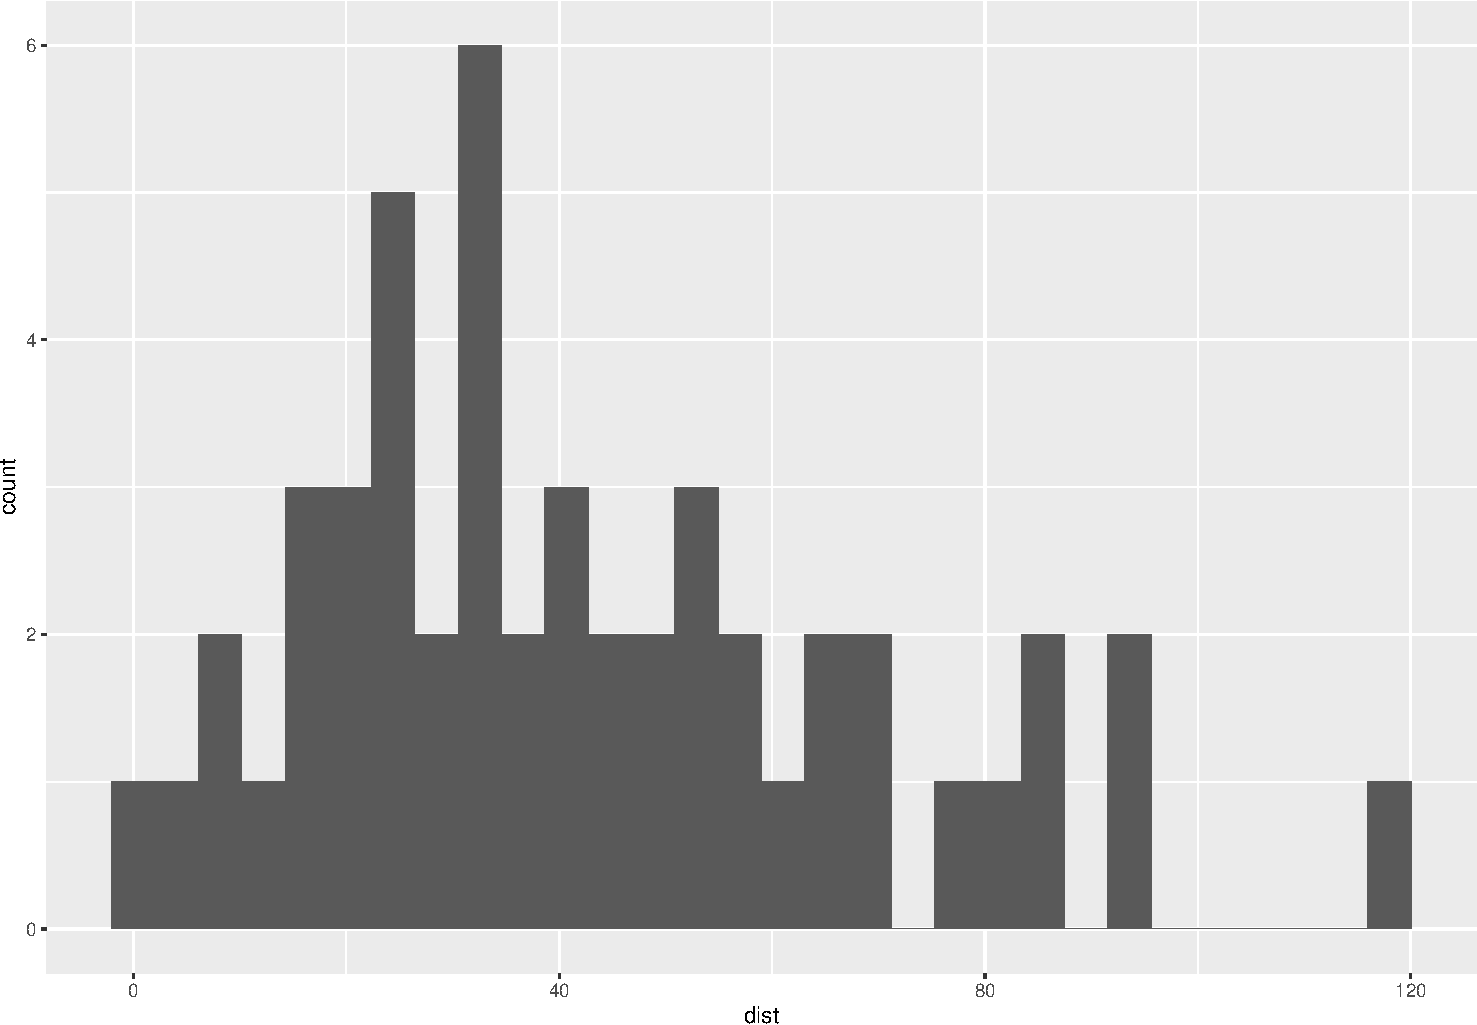
\includegraphics{Tema06_files/figure-beamer/unnamed-chunk-2-2.pdf}\end{minipage}%

\end{figure}%
\end{frame}

\begin{frame}[fragile]{Opciones globales para todas las celdas}
\phantomsection\label{opciones-globales-para-todas-las-celdas}
\begin{itemize}
\item
  Si no se da un valor a las opciones en una celda, se usa el valor por
  defecto de Quarto o el definido globalmente en la cabecera.
\item
  En la cabecera, se pueden especificar las opciones de ejecución de
  código \texttt{echo}, \texttt{eval}, \texttt{include},
  \texttt{output}, \texttt{error}, etc. en \texttt{execute} (ver
  \href{https://quarto.org/docs/reference/formats/html.html\#execution}{aquí}
  y \href{https://quarto.org/docs/computations/r.html}{aquí})

\begin{verbatim}
  ---
  execute:
    echo: false
    warning: false
  ---
\end{verbatim}
\end{itemize}

\begin{itemize}
\tightlist
\item
  También se pueden fijar en la cabecera muchas otras opciones,
  incluidas algunas que ya hemos visto (un listado completo
  \href{https://quarto.org/docs/reference/formats/html.html}{aquí para
  \texttt{html}})
\end{itemize}
\end{frame}

\begin{frame}[fragile]{Opciones por defecto para todas las celdas
(cont.)}
\phantomsection\label{opciones-por-defecto-para-todas-las-celdas-cont.}
\begin{verbatim}
    ---
    format:
      html:
        code-fold: true
        cap-location: bottom
        fig-align: center
        df-print: paged
    ---
\end{verbatim}

\begin{itemize}
\tightlist
\item
  La opción \texttt{df-print} especifica el método para visualizar
  tablas
\end{itemize}

\begin{itemize}
\tightlist
\item
  También se pueden especificar algunas de estas opciones a través del
  renderizador de R
  \href{https://quarto.org/docs/computations/r.html\#knitr-options}{\texttt{knitr}}
  (descripción completa
  \href{https://bookdown.org/yihui/rmarkdown/html-document.html}{aquí}).
\end{itemize}
\end{frame}

\begin{frame}{Ejecución de código en un documento .qmd}
\phantomsection\label{ejecuciuxf3n-de-cuxf3digo-en-un-documento-.qmd}
\begin{itemize}
\item
  Al renderizar un documento .qmd, se crea un nuevo espacio de trabajo y
  se ejecuta el código allí.

  \begin{itemize}
  \item
    ese espacio de trabajo es \emph{distinto} del que vemos en RStudio:
    diferentes objetos, incluyendo bibliotecas
  \item
    el directorio de trabajo también es diferente: es el directorio
    donde se encuentra el .qmd
  \end{itemize}
\item
  Es importante conocer si el código del documento .qmd ofrece los
  resultados deseado antes de renderizar.
\item
  Cuando tenemos varias celdas de código, algunas pueden depender de
  cálculos y objetos previos (datos, bibliotecas, resultados)
\end{itemize}

\begin{itemize}
\tightlist
\item
  Se puede probar ejecutando el código del documento .qmd (sin
  renderizar): línea a línea, la celda completa con
  
\includegraphics{figure/RunChunk.jpg} o todas las anteriores con
  
\includegraphics{figure/RunPrevChunk.jpg}
\end{itemize}
\end{frame}

\begin{frame}[fragile]{Ejecución de código en un .qmd (cont.)}
\phantomsection\label{ejecuciuxf3n-de-cuxf3digo-en-un-.qmd-cont.}
\begin{itemize}
\item
  Cuando ejecutamos el código sin renderizar, éste pasa pasa a la
  consola y \emph{sí} forma parte del espacio de trabajo de la sesión
  actual de R.
\item
  Debemos asegurarnos de que la sesión actual incluye sólo resultados
  del código de celdas del documento para que nuestra prueba sea
  equivalente a lo que obtendríamos renderizando
\item
  Resulta útil incluir una celda código al principio del documento (que
  se evalúe pero no muestre código ni resultados) que incluya

  \begin{itemize}
  \item
    \texttt{rm(list\ =\ ls())}: al ejecutar todas las celdas previas,
    empezamos con una sesión sin objetos y podemos probar el código de
    la celda actual
  \item
    Todas las bibliotecas (ej., \texttt{tidyverse}) que utilizaremos en
    varias celdas
  \item
    Fijar el directorio de trabajo para acceder a archivos (p.e.,
    imágenes, datos). Esto es innecesario si hemos sido cuidadosos y
    creado el archivo .qmd como parte de un proyecto.
  \end{itemize}
\end{itemize}
\end{frame}

\begin{frame}[fragile]{Mejorar la salida de tablas}
\phantomsection\label{mejorar-la-salida-de-tablas}
\begin{itemize}
\item
  Los resultados de muchas funciones de R no son visualmente
  ``profesionales'' en el documento de salida de .qmd
\item
  Varias bibliotecas cambian algunas salidas por defecto
  (\texttt{printr}) u ofrecen funciones para mejorarlas
  (\texttt{pander::pandoc.table()}, \texttt{xtable::xtable()})
\end{itemize}

\begin{itemize}
\item
  Por ahora, veremos la función \texttt{kable()} de la biblioteca
  \texttt{knitr}
\item
  Más adelante veremos la biblioteca \texttt{kableExtra}, con
  \href{https://cran.r-project.org/web/packages/kableExtra/vignettes/awesome_table_in_html.html}{más
  opciones}.

  \begin{itemize}
  \item
    \texttt{kableExtra} muestra ``data frame''/``tibbles'' como tablas
  \item
    \texttt{broom::tidy()} (de \texttt{tidyverse}) convierte mucho
    objetos de R (como listas con resultados de comandos) en
    \emph{tibbles}
  \end{itemize}
\end{itemize}

\begin{itemize}
\tightlist
\item
  Otras bibliotecas similares: \texttt{modelsummary}, \texttt{stargazer}
\end{itemize}
\end{frame}

\begin{frame}[fragile]{Comentarios finales: \emph{Dashboards}
(Tableros)}
\phantomsection\label{comentarios-finales-dashboards-tableros}
\begin{itemize}
\item
  Los \emph{dashboards} son un tipo de interfaz gráfica para los
  usuarios finales que ofrecen visualizaciones rápidas de indicadores o
  resultados clave
\item
  Estas presentaciones visuales e interactivas de los resultados de un
  análisis de datos puede ayudar a una comunicación más efectiva
\item
  Con Quarto se pueden crear varios tipos de
  \href{https://quarto.org/docs/interactive/}{\emph{dashboards}
  interactivos}, aunque no vamos a profundizar en ellos
\item
  En particular, Quarto trabaja con el paquete de R llamado
  \texttt{Shiny} que permite crear fácilmente aplicaciones web
  interactivas
\item
  Podéis encontrar ejemplos de las capacidades de \texttt{Shiny} en esta
  \href{https://shiny.rstudio.com/gallery/}{galería de aplicaciones}
\end{itemize}
\end{frame}

\begin{frame}[fragile]{Comentarios finales: libros de notas Jupyter}
\phantomsection\label{comentarios-finales-libros-de-notas-jupyter}
\begin{itemize}
\item
  Son otra forma de combinar texto, código y resultados en un documento
\item
  Desarrollados para \texttt{Python}, admiten varios lenguajes de
  programación

  \begin{itemize}
  \tightlist
  \item
    Quarto puede incluir celdas de código en otros lenguajes, incluido
    \texttt{Python}
  \end{itemize}
\item
  Se crean, visualizan y ejecutan solo en navegadores web, aunque son
  fácilmente modificables, en su entorno de trabajo

  \begin{itemize}
  \item
    con una \href{https://jupyter.org/install}{instalación local}
    (usando Python) u \emph{online} en
    \href{https://jupyter.org/try}{\textbf{JupyterLab}} (y también
    incluye un tipo de \emph{dashboard} propio: Voilà)
  \item
    o con \href{https://colab.research.google.com/}{Google Colab},
    también
    \href{https://colab.research.google.com/\#create=true&language=r}{para
    R}
  \end{itemize}
\item
  Quarto renderiza libros de Jupyter, creados en .qmd o en su propio
  formato
\item
  Muchas herramientas están preparadas para \texttt{Python} y \texttt{R}
  porque se usan a menudo indistintamente o combinados
\end{itemize}
\end{frame}



\end{document}
